% =====================================================================
% PAPER BODY: Methodology through Future Work.
%
% Generated by merge_paper.py. Do not edit both this file and
% paper_draft_methods_results.tex; this one supersedes it. The old
% Results section has been replaced with the real numbers.
%
% PREAMBLE (add before \begin{document}):
%   \usepackage{graphicx}
%   \graphicspath{{figures/}{figs/}{figured/}{./}}
%
% FIGURES to upload: fig_method.png, fig_scale.png,
%                    fig_beforeafter.png, fig_difficulty.png
%
% If your paper is SINGLE-column, change the figure* environment around
% fig_method.png to figure, and \textwidth to \linewidth.
% =====================================================================

\section{Methodology}

\begin{figure*}[t]
\centering
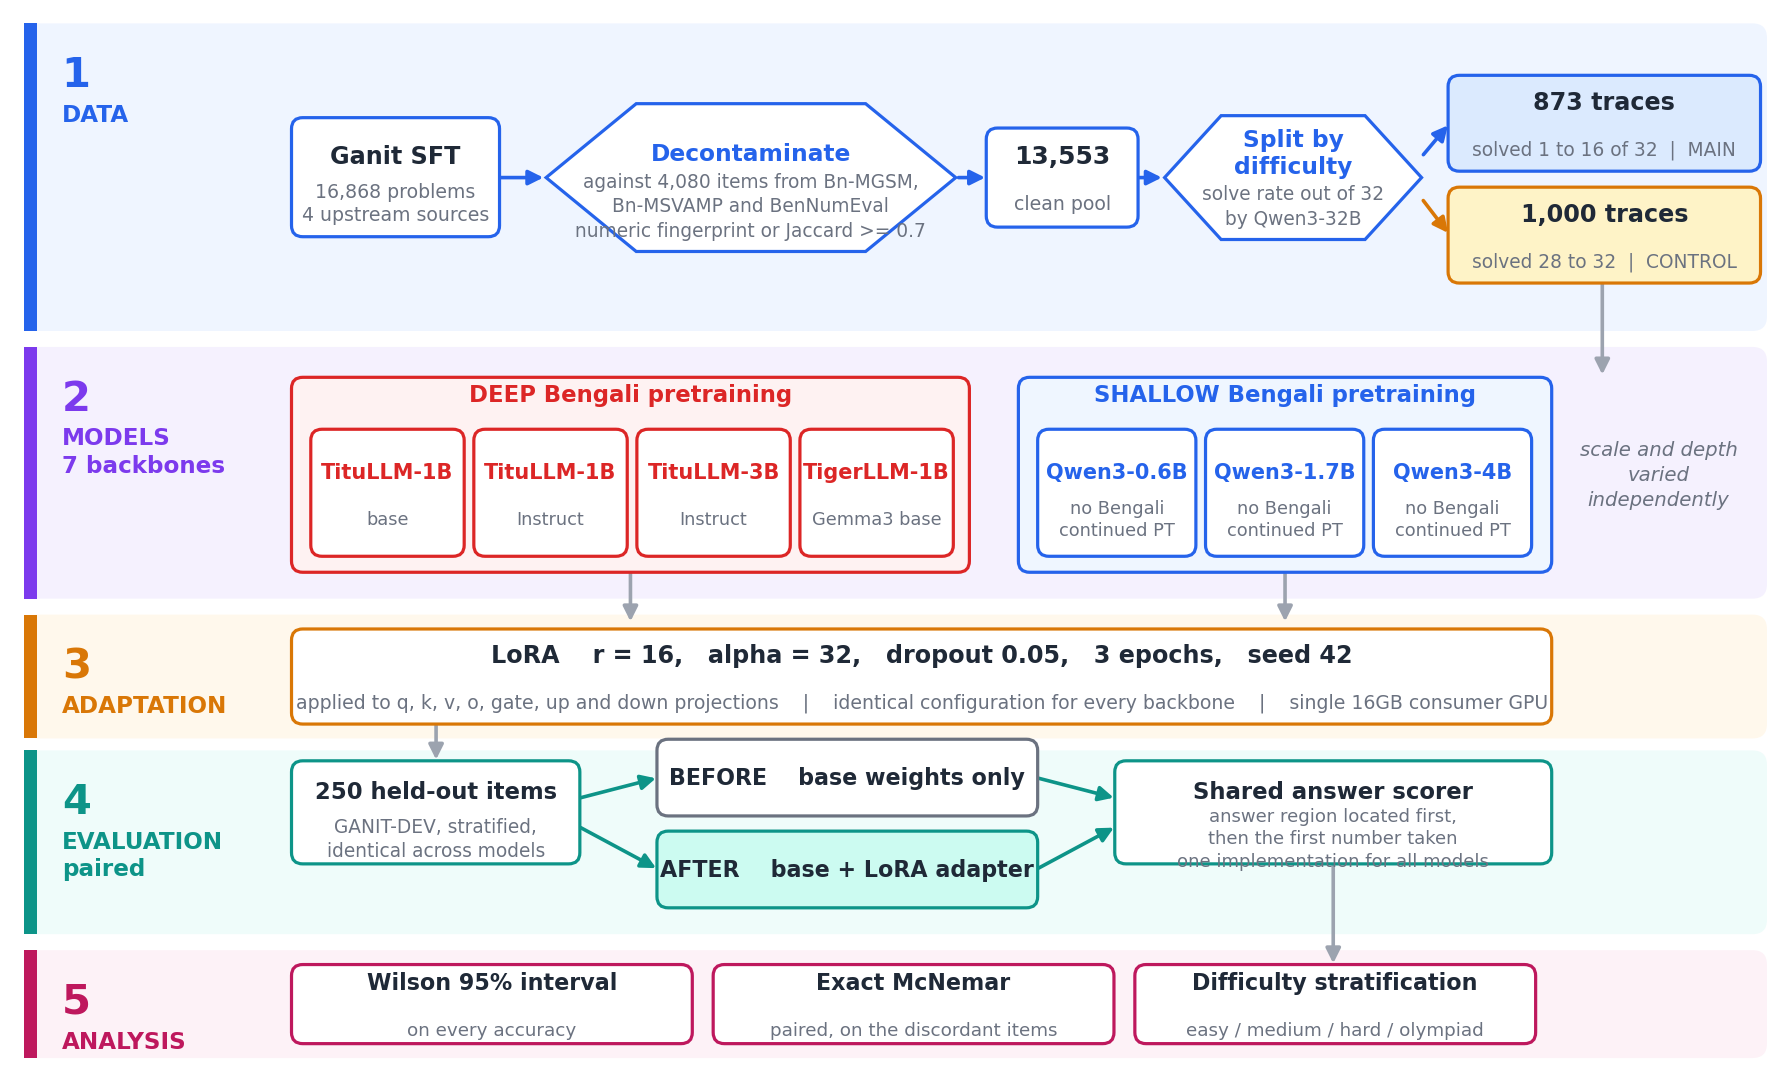
\includegraphics[width=\textwidth]{fig_method.png}
\caption{The study in full. Decontamination against three public Bengali
mathematics benchmarks precedes difficulty filtering, so the LIMO window is
applied to an already-clean pool. The two training sets differ only in the
difficulty band they are drawn from. Every backbone receives the identical
LoRA configuration and is evaluated on the identical held-out items in both
conditions, which makes every comparison in this paper a paired one.}
\label{fig:method}
\end{figure*}

\subsection{Experimental Design}

The study is a controlled experiment with two independent variables, parameter
scale and targeted Bengali pretraining depth, and one intervention, LIMO-style
minimal-data fine-tuning. Every model is evaluated twice on the same held-out
problems, once as released and once after fine-tuning, so each model acts as its
own control.

Seven backbones were selected so that the two independent variables move
separately. Table~\ref{tab:models} summarises them. TigerLLM-1B and TituLLM-1B
are close in size but differ by roughly $3{,}700\times$ in targeted Bengali
pretraining. TituLLM-1B and TituLLM-3B share a pretraining recipe and differ
only in size. The Qwen3 family spans 0.6B to 4B with no Bengali-specific
pretraining, isolating scale.

Two of the Bengali models are available in both base and instruction-tuned
form. Because TigerLLM is instruction-tuned and TituLLM's base models are not, a
comparison between them would confound pretraining depth with instruction
tuning. We therefore evaluate the instruction-tuned TituLLM variants as the
primary depth comparison and retain the base variants as an instruction-tuning
ablation.

\begin{table}[htbp]
\caption{The seven backbones under test. Bengali depth records whether the model received Bengali-specific continued pretraining beyond a general multilingual mix. Parameter counts are total, not trainable; LoRA trains roughly 0.5\% of them.}
\label{tab:models}
\centering
\begin{tabular}{|l|l|c|c|}
\hline
\textbf{Model} & \textbf{Base} & \textbf{Bengali PT} & \textbf{Params} \\
\hline
TigerLLM-1B-it        & Gemma3      & $\sim$10M tokens & 1.0B \\
TituLLM-1B v2.0       & Llama-3.2   & $\sim$37B tokens & 1.2B \\
TituLLM-1B-Instruct   & Llama-3.2   & $\sim$37B tokens & 1.2B \\
TituLLM-3B v2.0       & Llama-3.2   & $\sim$37B tokens & 3.2B \\
TituLLM-3B-Instruct   & Llama-3.2   & $\sim$37B tokens & 3.2B \\
Qwen3-0.6B            & Qwen3       & incidental       & 0.6B \\
Qwen3-1.7B            & Qwen3       & incidental       & 1.7B \\
Qwen3-4B              & Qwen3       & incidental       & 4.0B \\
\hline
\end{tabular}
\end{table}

\subsection{Training Data Curation}

Training data was drawn from the SFT split of the Ganit dataset
\parencite{ganitllm}, a Bengali mathematical reasoning corpus of 16,868
problems, each carrying a full Bengali reasoning trace and a difficulty score.
The difficulty score is the number of times Qwen3-32B solved the problem across
32 sampled attempts, so it records difficulty relative to a 32B model. The pool
is assembled from four upstream sources: numina-math-cot-bn (13,160 problems),
SOMADHAN (3,487), mCoT-MATH-bn (193) and s1k-32-Bangla (28). Its own difficulty
tags skew easy (10,065 easy, 6,411 olympiad, 258 hard, 134 medium), but the
solve-rate column tells a harsher story: 5,645 problems, a third of the corpus,
were never solved by Qwen3-32B in any of 32 attempts, and 91.7\% of that
unsolvable band comes from numina-math-cot-bn alone. We treat the zero band as
unreliable rather than merely hard, and exclude it.

Figure~\ref{fig:method} shows the pipeline. Decontamination ran first, before
any difficulty filtering, against 4,080 problems pooled from three public
Bengali mathematics benchmarks: Bn-MGSM (250 problems), Bn-MSVAMP (1,000) and
BenNumEval (2,830 across five task types). A training problem was removed if it
matched a benchmark problem on either of two signals. The first is a numeric
fingerprint, the hash of the sorted set of numbers appearing in the normalised
problem text. Numbers survive re-translation even when every surrounding word
changes, so this catches exactly the case that n-gram or MinHash deduplication
misses. The second is token Jaccard overlap at a threshold of 0.7, which
catches near-identical wording. Normalisation maps Bengali numerals to Western
digits, lowercases, strips punctuation and collapses whitespace, so the two
numeral conventions present in the corpus compare on equal footing. Together
these removed 3,315 problems and left 13,553.

Following LIMO's selection criterion, we then retained problems in the window
$1 \leq \text{correct\_counts} \leq 16$, which reduced 13,553 to 873. A final
near-duplicate pass within the surviving set removed nothing, which is itself
mild evidence that the pool is not padded with reworded repeats. The resulting
set is heavily weighted towards hard problems: 74.6\% carry an olympiad
difficulty tag and 25.3\% are tagged hard, with a mean pass rate of 3.3 out of
32.

A second training set was constructed later to test whether that difficulty
distribution explains our results. Holding every other choice constant, we
selected 1,000 traces from the band $\text{correct\_counts} \geq 28$, giving a
mean pass rate of 31.8 out of 32 and a difficulty composition of 100\% easy.
Section~\ref{sec:difficulty} reports that experiment. This set was
decontaminated directly against the held-out evaluation items rather than
against the public benchmarks, using the same numeric fingerprint idea. That
filter is deliberately aggressive and removed 1,782 candidates.

The evaluation set was independently checked against the 873 training traces by
identifier match, exact normalised text match, and numeric fingerprint combined
with Jaccard overlap. One item matched and was dropped. Neither training set
shares an identifier or problem text with the evaluation set, and the two
training sets are disjoint from each other because they are drawn from
non-overlapping difficulty bands. One limitation is worth stating plainly:
Ganit carries no upstream English source identifiers, so fingerprint and
Jaccard matching are proxies, and a sufficiently free paraphrase could survive
both filters.


\subsection{Evaluation Set}

The held-out set is 500 problems sampled from GANIT-DEV with seed 42,
stratified by difficulty: 145 easy, 127 medium, 129 hard and 99 olympiad. Gold
answers are short final values rather than worked solutions.

Compute constraints on a single consumer GPU limited scoring to the first 250
items of that shuffled set for every model, and to the first 100 for TituLLM-1B
base, which was withdrawn from the extension after producing degenerate output
at 0 to 2\% accuracy across its first hundred items. Every number in this paper
is therefore reported on 250 items unless stated otherwise. Because the set was
shuffled before truncation, the scored subset preserves the difficulty mix: 69
easy, 69 medium, 67 hard and 45 olympiad. All models see the same items in the
same order, so every before-and-after comparison in this paper is paired.

\subsection{Fine-Tuning Protocol}

All models were fine-tuned with LoRA \parencite{hu2021lora} using an identical
configuration: rank 16, $\alpha=32$, dropout 0.05, applied to the attention and
MLP projection matrices (\texttt{q\_proj}, \texttt{k\_proj}, \texttt{v\_proj},
\texttt{o\_proj}, \texttt{gate\_proj}, \texttt{up\_proj}, \texttt{down\_proj}).
Training used a learning rate of $2\times10^{-4}$ with cosine decay and 3\%
warmup, three epochs, per-device batch size 1 with gradient accumulation 16 for
an effective batch of 16, bfloat16 precision, gradient checkpointing, and seed
42. Loss was computed on the target tokens only, with prompt tokens masked.

The training target is the full Bengali reasoning trace from the Ganit
\texttt{messages} field, not the short final answer. Training on the bare answer
would teach the model to emit a value and stop, which is close to the opposite
of reasoning elicitation.

The Bengali instruction text is byte-identical for every model. Only the wrapper
around it differs: completion-style models receive the instruction followed by a Bengali
solution cue (\emph{somadhan}, meaning ``solution''), while instruction-tuned
models receive it through their own chat template. This choice was made empirically rather than assumed. We probed
both formats on each model and selected whichever produced a lower token-cap
rate, on the reasoning that a format a model was never trained in prevents it
from terminating. For Qwen3 models, thinking mode was disabled so that every
backbone receives the same intervention.

All experiments ran on a single NVIDIA RTX 5060 Ti with 16GB of VRAM. Total
training time across all adapters was approximately 4.4 GPU-hours.

\subsection{Availability and Computational Environment}

All experiments ran under Python 3.11.16 with PyTorch 2.8.0+cu128,
Transformers 4.57.6 and PEFT 0.20.0, on a single NVIDIA RTX 5060 Ti with 16GB
of VRAM. Seed 42 was set for Python, NumPy and PyTorch in every run, and all
generation is greedy, so no sampling randomness enters the results.
Deterministic CUDA algorithms were not enabled, because the throughput cost was
prohibitive on this hardware; the consequence is that training losses reproduce
to roughly three decimal places rather than exactly, while greedy generations
are stable.

The curation notebook, the training and evaluation harness, the shared answer
scorer with its executable test suite, and the analysis scripts that regenerate
every table, figure and reported number in this paper from the stored model
outputs are available at [REPOSITORY URL]. The exact environment record,
including package versions and the reproducibility caveats above, is committed
as \texttt{environment.json}.

\subsection{Evaluation Protocol}

Generation is greedy, with a repetition penalty of 1.1 and a per-model
generation budget set to the 99th percentile of that model's own training-target
length. This last point matters and is not a detail. An equal token budget is
not an equal opportunity when tokenizers differ by a factor of three. The same
873 Bengali traces require a median of 397 tokens under TituLLM's tokenizer, 428
under TigerLLM's, and 1,245 under Qwen3's. A uniform 1,024-token cap would leave
the Bengali models room to spare while truncating 42\% of what Qwen3 was trained
to produce. Qwen3 models therefore receive 2,048 tokens and the Bengali models
1,024, with the budget recorded for every prediction.

Generation halts on any end-of-sequence marker the tokenizer knows, rather than
only its declared \texttt{eos\_token}. This is necessary because TituLLM
declares \texttt{<|eot\_id|>}, a chat turn terminator, while being prompted in
completion format where that token never follows free text. Under a
single-token stopping rule the model has no reachable way to stop.

\subsection{Answer Extraction and Scoring}

Answers are scored by exact match after normalisation. Extraction proceeds by
narrowing to an answer region, using \texttt{<answer>} tags, then
\texttt{\textbackslash boxed\{\}}, then the Bengali answer marker \emph{uttar}
(``answer''), and finally the last numeral in the generation, before taking the
first numeric token inside that region. Normalisation maps Bengali numerals
to ASCII, strips currency, percentage and LaTeX markup, and compares numerically
where possible.

Taking the first number inside the answer region rather than the whole region is
essential. An earlier version returned the entire remainder of the line after
the answer marker. A correct answer written naturally, for example
\emph{uttar}: 20 \emph{jon chhatro} (``answer: 20 students''), was compared in
full against a gold value of 20, failed to normalise, and was scored wrong even
though the model was right. The scorer is distributed with an executable
test suite built from verbatim model outputs rather than synthetic cases.

Generations that produce no parseable answer are recorded as format failures and
reported separately from wrong answers.

\subsection{Statistical Analysis}

Because every model is evaluated on the same items, before-and-after comparisons
are paired and use the exact McNemar test on discordant pairs. Comparisons
between different models use Fisher's exact test. Proportions are reported with
Wilson score intervals, which behave correctly near zero where the normal
approximation does not. Continuous measures such as generation length and
Bengali character ratio are reported as mean paired differences with 95\%
confidence intervals, and treated as significant when the interval excludes
zero.

Every before-and-after comparison is reported with a paired risk difference
$\Delta$ and its 95\% confidence interval alongside the $p$-value, because a
$p$-value alone says whether an effect is distinguishable from zero but not how
large it could plausibly be. Where the two disagree we treat the exact test as
authoritative: the Wald interval on a paired difference is anti-conservative
when the discordant counts are very small, which happens here for
TituLLM-1B-Instruct with eight discordant pairs.

We report significance tests rather than raw differences throughout because
accuracies in this study are low. At 3\% accuracy on 250 items, a difference of
three correct answers looks like a trend and is not one.

No correction for multiple comparisons is applied. Seven McNemar tests, three
Fisher tests and seven sign tests are reported. Since every McNemar result is
null, a correction could only make them more null and would not change any
conclusion; the Fisher and sign-test results survive Bonferroni correction at
$\alpha=0.05$ by several orders of magnitude. Readers should nonetheless treat
the single borderline value, $p=0.070$ for TituLLM-1B-Instruct, as weaker than
it looks in isolation.


% =====================================================================

\section{Results}
\label{sec:results}

\subsection{Scale Predicts Bengali Reasoning; Pretraining Depth Does Not}
\label{sec:rq1}

Figure~\ref{fig:scale} is the central result. Plotting untuned accuracy against
parameter count separates the models cleanly into two regimes, and the
separating variable is not the one the field's Bengali-specific model releases
would predict.

\begin{figure}[htbp]
\centering
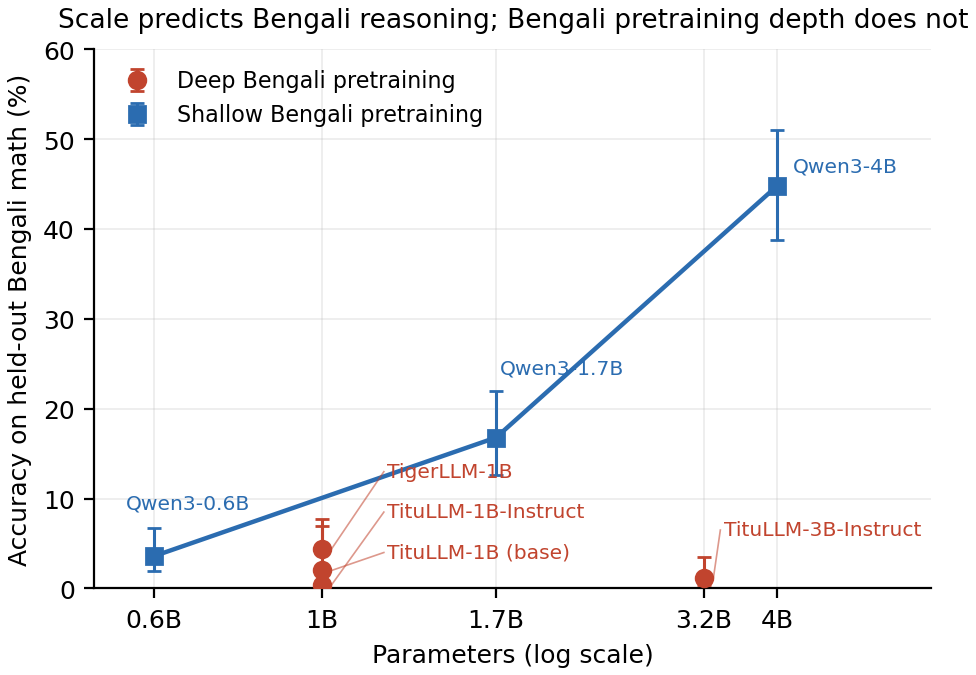
\includegraphics[width=\linewidth]{fig_scale.png}
\caption{Exact-match accuracy on held-out Bengali mathematics word problems,
plotted against total parameter count, for all seven backbones as released and
before any fine-tuning. Each model is scored on the same 250 items (100 for
TituLLM-1B base); vertical bars are Wilson 95\% intervals and the horizontal
axis is logarithmic. The line joins members of the Qwen3 family and is a visual
guide, not a fitted trend. Notice that the four models with deep Bengali
pretraining sit flat near the floor across a threefold range of parameters,
while the three with only incidental Bengali coverage climb steeply with
scale.}
\label{fig:scale}
\end{figure}

Within the Qwen3 family, which received no Bengali-specific pretraining beyond
whatever appears in a general multilingual mix, accuracy rises monotonically
and steeply: 3.6\% at 0.6B, 16.8\% at 1.7B, and 44.8\% at 4B. Every adjacent
step is significant under an unpaired Fisher exact test: $p=1.0\times10^{-6}$
from 0.6B to 1.7B, $p=1.3\times10^{-11}$ from 1.7B to 4B, and
$p=7.4\times10^{-30}$ across the full ladder. That is better than an order of
magnitude of improvement across less than one order of magnitude of
parameters.

The Bengali-specialised models show no such gradient. TituLLM-1B-Instruct
reaches 0.4\%, TituLLM-1B base 2.0\%, TigerLLM-1B 4.4\%, and TituLLM-3B-Instruct
1.2\%. Tripling the parameter count from 1B to 3.2B buys nothing. All four sit
inside each other's confidence intervals and all four sit near the floor.

The sharpest single comparison is TituLLM-3B-Instruct against Qwen3-1.7B.
TituLLM-3B-Instruct has roughly twice the parameters and was continually
pretrained on a large Bengali corpus with a tokenizer extended for the
language. Qwen3-1.7B has neither advantage. Qwen3-1.7B scores 16.8\% against
TituLLM-3B-Instruct's 1.2\% (Fisher exact, $p=1.7\times10^{-10}$). The
advantage is not an artifact of one difficulty tier. The smaller, Bengali-shallow model wins at easy (17.4\% against 1.4\%),
medium (20.3\% against 1.4\%), hard (13.4\% against 1.5\%) and olympiad (15.6\%
against 0.0\%) alike.

This answers RQ1 directly, and answers it in the negative. Targeted Bengali
pretraining depth, as delivered by the two publicly released Bengali model
families we could obtain, does not substitute for scale on mathematical
reasoning. Whatever those models gained from Bengali continued pretraining, and
they did gain something, since their tokenizers are far more efficient on
Bengali text, it did not transfer into mathematical competence.

\subsection{Minimal-Data Elicitation Moves No Model}
\label{sec:rq1b}

Table~\ref{tab:main} and Figure~\ref{fig:beforeafter} report the paired
before-and-after comparison for all seven backbones.

We report accuracy rather than precision, recall or F1 because the task is
free-form generation of a numeric answer scored by exact match, not
classification: there are no classes over which those metrics are defined and
no confusion matrix to construct. In their place we report the diagnostics that
do carry information for generative scoring, namely format-failure rate,
token-cap rate, language adherence, per-difficulty accuracy
(Table~\ref{tab:difficulty}) and answer retention
(Table~\ref{tab:retention}).

% Regenerate every table with:  python paper_stats.py
\begin{table*}[t]
\caption{Accuracy before and after LIMO-style fine-tuning on 873 curated
Bengali reasoning traces, on the same 250 held-out items per model
(TituLLM-1B base on 100). Intervals on each accuracy are Wilson 95\%.
$\Delta$ is the paired risk difference in percentage points with its 95\%
confidence interval; it is the effect size, and it is reported because a
$p$-value alone does not bound how large the change could be. $p$ is a
two-sided exact McNemar test on the discordant pairs. Notice that every
$\Delta$ interval contains zero.}
\label{tab:main}
\centering\small
\begin{tabular}{|l|c|c|c|c|c|c|c|c|}
\hline
\textbf{Model} & \textbf{Params} & \textbf{Bn depth} & \textbf{$n$} & \textbf{Before} & \textbf{After} & \textbf{$\Delta$ (pp)} & \textbf{95\% CI} & \textbf{$p$} \\
\hline
TituLLM-1B (base) & 1.0B & deep & 100 & 2.0\% & 0.0\% & -2.0 & [-4.7, +0.7] & 0.500 \\
TituLLM-1B-Instruct & 1.0B & deep & 250 & 0.4\% & 2.8\% & +2.4 & [+0.2, +4.6] & 0.070 \\
TigerLLM-1B & 1.0B & deep & 250 & 4.4\% & 2.4\% & -2.0 & [-4.8, +0.8] & 0.267 \\
TituLLM-3B-Instruct & 3.2B & deep & 250 & 1.2\% & 1.2\% & +0.0 & [-1.9, +1.9] & 1.000 \\
Qwen3-0.6B & 0.6B & shallow & 250 & 3.6\% & 6.0\% & +2.4 & [-0.7, +5.5] & 0.210 \\
Qwen3-1.7B & 1.7B & shallow & 250 & 16.8\% & 18.0\% & +1.2 & [-4.4, +6.8] & 0.780 \\
Qwen3-4B & 4.0B & shallow & 250 & 44.8\% & 39.6\% & -5.2 & [-13.0, +2.6] & 0.228 \\
\hline
\end{tabular}
\end{table*}

\begin{table*}[t]
\caption{Accuracy by difficulty tier, before and after fine-tuning, for
every backbone on the same held-out items. Tier counts are 69 easy, 69
medium, 67 hard and 45 olympiad for the models evaluated on 250 items,
and 30/24/29/17 for TituLLM-1B base on 100. Notice that the Qwen3
advantage holds in every tier rather than coming from one band, and that
no tier shows a consistent post-tuning gain.}
\label{tab:difficulty}
\centering\small
\begin{tabular}{|l|c|c|c|c|}
\hline
\textbf{Model} & \textbf{Easy} & \textbf{Medium} & \textbf{Hard} & \textbf{Olympiad} \\
\hline
TituLLM-1B (base) & 0.0 $\rightarrow$ 0.0 & 4.2 $\rightarrow$ 0.0 & 3.4 $\rightarrow$ 0.0 & 0.0 $\rightarrow$ 0.0 \\
TituLLM-1B-Instruct & 1.4 $\rightarrow$ 5.8 & 0.0 $\rightarrow$ 2.9 & 0.0 $\rightarrow$ 1.5 & 0.0 $\rightarrow$ 0.0 \\
TigerLLM-1B & 7.2 $\rightarrow$ 2.9 & 4.3 $\rightarrow$ 2.9 & 1.5 $\rightarrow$ 3.0 & 4.4 $\rightarrow$ 0.0 \\
TituLLM-3B-Instruct & 1.4 $\rightarrow$ 1.4 & 1.4 $\rightarrow$ 1.4 & 1.5 $\rightarrow$ 1.5 & 0.0 $\rightarrow$ 0.0 \\
Qwen3-0.6B & 2.9 $\rightarrow$ 8.7 & 4.3 $\rightarrow$ 4.3 & 4.5 $\rightarrow$ 9.0 & 2.2 $\rightarrow$ 0.0 \\
Qwen3-1.7B & 17.4 $\rightarrow$ 21.7 & 20.3 $\rightarrow$ 20.3 & 13.4 $\rightarrow$ 19.4 & 15.6 $\rightarrow$ 6.7 \\
Qwen3-4B & 59.4 $\rightarrow$ 55.1 & 44.9 $\rightarrow$ 34.8 & 40.3 $\rightarrow$ 40.3 & 28.9 $\rightarrow$ 22.2 \\
\hline
\end{tabular}
\multicolumn{1}{l}{\small All values are percentages, before $\rightarrow$ after.}
\end{table*}

\begin{figure}[htbp]
\centering
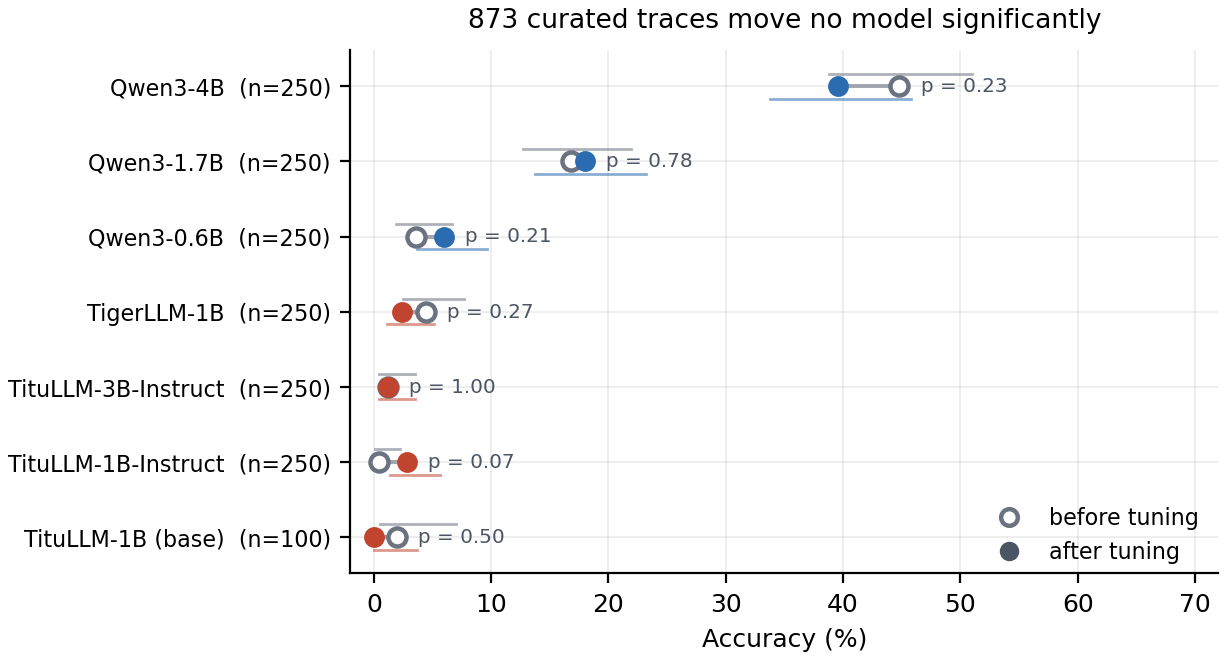
\includegraphics[width=\linewidth]{fig_beforeafter.png}
\caption{Exact-match accuracy for each backbone before and after LoRA
fine-tuning on the same 873 curated Bengali traces, scored on the same held-out
items in both conditions ($n=250$; $n=100$ for TituLLM-1B base). Hollow markers
are the untuned model, filled markers the adapter, and the thin lines behind
each marker are Wilson 95\% intervals. $p$ values are two-sided exact McNemar
tests on the discordant pairs. Notice that the intervals for the two conditions
overlap substantially for every model, and that no comparison crosses the 0.05
threshold.}
\label{fig:beforeafter}
\end{figure}

Not one of the seven comparisons reaches significance. The smallest $p$ value in
the table is 0.070, for TituLLM-1B-Instruct, on a change from 0.4\% to 2.8\%
that amounts to six additional correct answers out of 250. Three models moved
up, three moved down, and one did not move at all. That distribution is what
noise looks like.

The result is worth stating carefully, because a null result invites two
different readings and only one of them is supported here. The reading we can
defend is that 873 curated traces do not elicit latent mathematical reasoning
in Bengali at the 0.6B to 4B scale. The reading we cannot defend is that
LIMO-style elicitation does not work, full stop. Our largest model is 4B.
\textcite{wei2022emergent} place the threshold for arithmetic emergence near
13B and for chain-of-thought benefit substantially higher, and every model in
this study sits below both. A negative result collected entirely below a
capability threshold is evidence about that region, not about the method.

Qwen3-4B is the one row where the point estimate moved by a visible margin, from
44.8\% down to 39.6\%. The direction survived the extension from 100 items to
250, but the significance did not arrive with it: 56 items were lost against 43
gained, giving $\Delta = -5.2$ percentage points with a 95\% confidence interval
of $-13.0$ to $+2.6$, and an exact McNemar $p=0.228$. The interval contains zero
and is wide enough to accommodate a modest gain, so we do not read a real
degradation into it. It is worth noting that this is the only model with
enough baseline accuracy for a degradation to have been visible at all.

\subsection{Output Behaviour Changed Even Though Accuracy Did Not}
\label{sec:behaviour}

The tuning was not inert. It changed what the models produced; it simply did not
change whether the produced answers were right.

The clearest case is TituLLM-1B base. Untuned, it hit the generation cap on
100\% of items, meaning it never once emitted a stop token and every completion
was truncated at the token budget. After fine-tuning on 873 traces, that fell to
47\%. The model learned, from a very small number of examples, what a finished
Bengali reasoning trace looks like and when to stop producing one. Its accuracy
over the same items went from 2.0\% to 0.0\%.

Across the other backbones the cap rate mostly moved the other way. It rose
after tuning for four of the seven models, most sharply for Qwen3-0.6B (4.8\%
to 36.8\%) and TituLLM-3B-Instruct (8.0\% to 29.2\%). Trained on long worked
solutions, those models produced longer outputs. They did not produce more
correct ones. Qwen3-4B is the informative exception: the one model with real
baseline competence barely moved on this measure at all, from 8.8\% to 7.6\%,
which is what we would expect from a model that already knew how to finish a
worked solution before it saw any of ours.

Stopping behaviour, then, moved in whichever direction the base model had the
most room to move in, and in no case did it move accuracy with it. The next
section takes this further and asks what the adapter changed at the level of
individual items.

\subsection{What the Fine-Tuning Actually Did}
\label{sec:retention}

A null result invites the objection that nothing happened at all: that the
adapter never took, or that LoRA at rank 16 is too small to move a model. The
item-level data rules that out. A great deal happened. It simply was not
learning to reason.

Table~\ref{tab:retention} reports answer retention, meaning the share of items
a model answered correctly before fine-tuning that it still answered correctly
afterwards. If 873 traces were teaching mathematical reasoning, retention
should be high and the gains should sit on top of it. That is not the pattern.

\begin{table}[htbp]
\caption{Answer retention. Of the items each model answered correctly
before fine-tuning, how many it still answered correctly afterwards, and
how many items changed outcome in either direction. Notice that no model
retained even half of what it already knew, which is why the small net
changes in Table~\ref{tab:main} understate how much the adapter moved.}
\label{tab:retention}
\centering\small
\begin{tabular}{|l|c|c|c|c|}
\hline
\textbf{Model} & \textbf{Correct before} & \textbf{Retained} & \textbf{Retention} & \textbf{Items flipped} \\
\hline
Qwen3-4B & 112 & 56 & 50\% & 99 / 250 \\
Qwen3-1.7B & 42 & 18 & 43\% & 51 / 250 \\
Qwen3-0.6B & 9 & 4 & 44\% & 16 / 250 \\
TigerLLM-1B & 11 & 2 & 18\% & 13 / 250 \\
TituLLM-3B-Instruct & 3 & 0 & 0\% & 6 / 250 \\
TituLLM-1B-Instruct & 1 & 0 & 0\% & 8 / 250 \\
\hline
\end{tabular}
\end{table}

Qwen3-4B answered 112 items correctly before tuning and kept 56 of them. It
also answered 43 items correctly that it had failed before. In total 99 of 250
items changed their outcome, close to 40\% of the evaluation set, while net
accuracy moved by 13 items. The same shape holds down the scale: no model
retained even half of what it already knew. The adapter did not add a layer of
competence on top of the base model. It substantially rewrote which problems
the model could solve, and the replacement set happened to be slightly worse
than the original.

The mechanism is visible in the generated text. Before fine-tuning, Qwen3-4B
closed 225 of 250 completions with the Bengali word for ``answer'' followed by
its result, a convention it adopted on its own, since the evaluation prompt
asks only that the model answer in Bengali and specifies no format. After
fine-tuning it did so on 3 of 250. In its place the model adopted the format of
the training corpus: Ganit's traces are written as a \texttt{<think>} block
followed by an \texttt{<answer>} block, and after tuning every one of the 250
completions opened a \texttt{<think>} block. Median output length fell from
1,046 tokens to 887, the proportion of Bengali characters fell from 87.0\% to
82.0\%, and the number of explicit step markers roughly halved.

This is the Superficial Alignment Hypothesis \parencite{zhou2023lima} observed
from the unfavourable side. In LIMA's setting a small number of examples
exposes capability the pretrained weights already hold, and the result is a
useful model. Here the same small number of examples reshaped format, length,
language mix and stopping behaviour just as comprehensively, and exposed
nothing, because at this scale there was little underneath to expose. Style
transferred completely. Reasoning did not transfer at all.

\subsubsection*{A sensitivity check on the format change}

Because the output format changed, it is worth confirming that the accuracy
drop is not an artifact of answer extraction. Our scorer looks for an
\texttt{<answer>} block first, then a boxed expression, then the Bengali answer
marker, and only if none of those are present does it fall back to taking the
last number in the completion. After fine-tuning, 230 of 250 Qwen3-4B
completions contained a well-formed \texttt{<answer>} block and were therefore
parsed by the strongest branch of the extractor. The remaining 20 exhausted the
generation budget inside the \texttt{<think>} block and were scored by the weak
fallback. Of the 56 items Qwen3-4B lost, 45 produced a well-formed
\texttt{<answer>} that was simply wrong. The failures are arithmetic, not
formatting. On one item with gold answer 16 the tuned model emitted
\texttt{<answer>0</answer>}; on another with gold 126 it emitted
\texttt{<answer>14</answer>}. In both cases the extractor read exactly what the
model wrote.

To bound the effect, we recomputed accuracy crediting every fallback-scored
item as correct, which is the most generous assumption available. Post-tuning
accuracy under that assumption is 46.8\%, against a measured 39.6\% and a
pre-tuning 44.8\%. The true value therefore lies somewhere between a loss of
5.2 points and a gain of 2.0 points. We cannot sign the effect, which is
consistent with the exact McNemar test returning $p=0.228$, and the substantive
conclusion is unchanged in either direction: 873 curated traces did not produce
a detectable improvement in Bengali mathematical reasoning at this scale.

\subsection{The Null Is Not a Difficulty-Calibration Artifact}
\label{sec:difficulty}

The most obvious objection to Section~\ref{sec:rq1b} is that our training set was
simply too hard. The LIMO window selects problems a 32B model solves between 1
and 16 times out of 32, which for a 1.7B model may be far outside the range it
can learn anything from. If so, the null would say more about our data selection
than about elicitation.

Figure~\ref{fig:difficulty} reports that test. Holding the backbone, the
LoRA configuration, the seed,
the prompt and the evaluation items constant, we built a second training set of
1,000 traces from the opposite end of the difficulty distribution, requiring at
least 28 correct out of 32, and trained the same Qwen3-1.7B on it.

\begin{figure}[htbp]
\centering
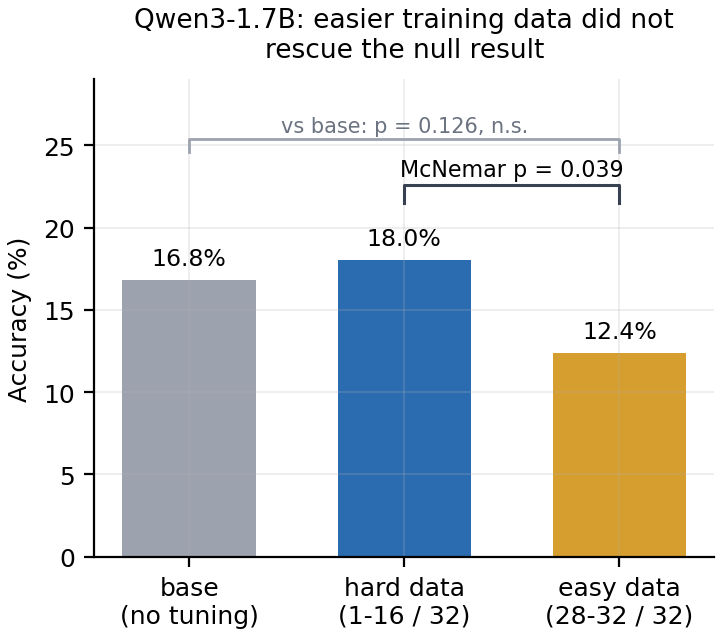
\includegraphics[width=0.72\linewidth]{fig_difficulty.png}
\caption{Qwen3-1.7B under three conditions, scored on the same 250 held-out
items, with backbone, LoRA configuration, seed, prompt and evaluation items
held fixed so that training-data difficulty is the only thing that varies. The
easy-data adapter is significantly worse than the hard-data adapter (exact
McNemar, $p=0.039$); against the untuned base it is lower but not significantly
so ($p=0.126$), as marked. Notice that easier, better-calibrated training data
did not rescue the null result and if anything moved accuracy the wrong way.}
\label{fig:difficulty}
\end{figure}

The easy-data adapter reached 12.4\%, against 18.0\% for the hard-data adapter
and 16.8\% for the untuned base. The gap between the two adapters is
significant (exact McNemar, 27 items lost against 13 gained, $p=0.039$), and it
runs in the opposite direction to the objection. Easier, better-calibrated
training data did not rescue the null. It made results worse.

Against the untuned base, by contrast, the easy-data adapter is lower but not
significantly so (12.4\% against 16.8\%, exact McNemar $p=0.126$). The claim we
can defend is the narrower one: easier data is significantly worse than harder
data, not that it is significantly worse than no tuning at all.

This closes the difficulty explanation. The models can learn from calibrated
data, and doing so does not improve held-out reasoning and may actively harm it.

\subsection{The Bengali Tokenizer Tax}
\label{sec:tokenizer}

One finding did come out clearly in favour of the Bengali-specialised models,
and it is a real one even though it did not translate into accuracy.
Table~\ref{tab:tokenizer} reports token counts for the same 873 training
traces under each tokenizer.

\begin{table}[htbp]
\caption{Tokens required to represent the same 873 training sequences
under each tokenizer, measured on the full sequence train\_lora.py
builds: shared Bengali instruction, problem, model-specific prompt
formatting, and reasoning trace. Vocabulary sizes include added tokens.
Notice that the two Bengali-adapted tokenizers need roughly a third as
many tokens as Qwen3 for identical content, and that this efficiency is
not reflected in the accuracies of Table~\ref{tab:main}.}
\label{tab:tokenizer}
\centering
\begin{tabular}{|l|c|c|c|c|}
\hline
\textbf{Tokenizer} & \textbf{Vocab} & \textbf{Median} & \textbf{p95} & \textbf{Max} \\
\hline
TituLLM-1B & 170,497 & 395 & 871 & 1,498 \\
TigerLLM-1B & 262,145 & 425 & 930 & 1,431 \\
Qwen3 & 151,669 & 1,244 & 2,395 & 3,543 \\
\hline
\end{tabular}
\end{table}

Qwen3 needs roughly $3.1\times$ more tokens than TituLLM to represent identical
Bengali text, close to the $3.5\times$ reported by
\textcite{yong2025crosslingual} and consistent with the per-model premiums in
\textcite{petrov2023language}.

The cost is concrete rather than theoretical. On a single 16GB consumer card it
determined which configurations were trainable at all. Qwen3-4B could not be
trained at a 4,096-token sequence limit and required a reduction to 2,048, which
truncated 104 of the 873 traces. No Bengali-tokenized model faced that
constraint. The same pressure appeared at inference: TituLLM-3B-Instruct pairs
3.2B parameters with a 170,497-token vocabulary, which makes the output logits
tensor the binding memory cost during generation and forced a batch size of one.

It is worth noting that TigerLLM's efficiency is inherited rather than earned.
Gemma3 ships a 262k vocabulary described as balanced for non-English languages
\parencite{gemma3}, and TigerLLM adds exactly one token to it. TituLLM, by
contrast, extended Llama-3.2's vocabulary deliberately for Bengali. Both end up
around three times more efficient than Qwen3 on this corpus, by quite different
routes.

The broader point is that tokenizer efficiency and downstream reasoning are
separable. The two most token-efficient models in this study are also the two
weakest at mathematics. Efficiency on Bengali text is necessary for practical
deployment on constrained hardware, and it is not sufficient for reasoning.


\section{Discussion}
\label{sec:discussion}

\subsection{What the Scale Result Means}

Our headline result contradicts TigerLLM's central claim, using TigerLLM's own
released model on a Bengali benchmark. That claim was that targeted,
high-quality pretraining can substitute for scale. We find that it does not, at
least for mathematical reasoning: a $3{,}700\times$ difference in Bengali
pretraining produced no measurable difference, while parameter scale produced a
large and monotonic one.

This is consistent with a literature that has been converging on the same point
from other directions. \textcite{kaplan2020scaling} found performance depends % NEW
strongly on scale and weakly on architectural choices. \textcite{wei2022emergent} % NEW
place the emergence of three-digit arithmetic at roughly 13B parameters and the
benefit of chain-of-thought on GSM8K at roughly 100B. MathMist
\parencite{sobhani2026mathmist} reports the Bengali-English gap closing as Qwen
scales. Our contribution is to separate the variables that this prior work left
entangled, in the one language where the substitution claim was made.

We are careful about what this does not show. It does not show that targeted
Bengali pretraining is worthless. TituLLM's extended tokenizer delivers a real,
measured threefold efficiency gain, and that gain determines what can be trained
on accessible hardware. It shows that targeted depth did not buy mathematical
reasoning.

\subsection{Why Elicitation Changed Form and Not Capability}

LIMA's Superficial Alignment Hypothesis \parencite{zhou2023lima} % NEW
holds that a model's knowledge comes almost entirely from pretraining and that
alignment mainly teaches formatting and style. Our results are a clean, if
unflattering, confirmation of exactly that. Fine-tuning taught these models to
open a reasoning block, to structure a worked solution, and in TituLLM's case to
stop generating at all. It did not teach them to arrive at correct answers.

Two mechanisms plausibly contribute, and we cannot fully separate them.

The first is capacity of the adaptation method. \textcite{biderman2024lora} % NEW
report that LoRA at rank 16, the configuration used here, reaches 0.158 on
GSM8K after continued pretraining where full fine-tuning reaches 0.293, and
conclude that low-rank settings substantially underperform full fine-tuning on
tasks requiring new capability. The first half of that description matches what
we observe.

The second half does not, and the difference is worth stating. Biderman et al.
also report that LoRA forgets less than full fine-tuning and stays closer to
base behaviour. Our retention data in Section~\ref{sec:retention} shows nothing
of the kind: no backbone kept even half of the items it had answered correctly,
and Qwen3-4B abandoned its own output format on 222 of 250 items. We did not
run full fine-tuning, so we cannot claim LoRA forgets more than the alternative.
What we can say is that rank 16 on 873 examples was more than sufficient to
overwrite a model's answering behaviour, and that the common intuition of a
low-rank adapter as a small, conservative edit does not describe this setting.

The second is the capability of the backbones themselves. If arithmetic
competence emerges above 13B \parencite{wei2022emergent}, % NEW
then LIMO's precondition may simply not hold in the 0.6B to 4B range regardless
of adaptation method. Qwen3-4B complicates this reading, since its baseline
accuracy of 44.8\% shows real latent capability, and elicitation still
produced nothing.

\subsection{The Bengali Adherence Decline}

The finding we did not anticipate is that training on Bengali reasoning traces
made models less Bengali. Six of the seven backbones produced a lower
proportion of Bengali characters after fine-tuning than before it. The
decline was sharpest in exactly the models that started most Bengali:
TituLLM-3B-Instruct fell from 97.9\% to 80.8\% and TituLLM-1B-Instruct from
98.3\% to 81.3\%. TigerLLM-1B fell from 87.0\% to 82.7\% and Qwen3-1.7B from
89.3\% to 84.1\%. Qwen3-0.6B was the single exception, rising slightly from
85.6\% to 87.8\%. Training on Bengali reasoning traces made most of these
models write less Bengali, not more.

Table~\ref{tab:adherence} reports the paired differences with their
95\% confidence intervals. In all six declining models the interval
excludes zero. Qwen3-0.6B is the exception in both directions: its mean
rose by 2.1 points but the interval spans zero ($-1.2$ to $+5.4$), so we
do not claim it improved, even though more of its individual items fell
than rose.

\begin{table*}[t]
\caption{Bengali character ratio in generated output, before and after
fine-tuning on Bengali reasoning traces. $\Delta$ is the mean paired
difference in percentage points with its 95\% confidence interval; $p$ is
a two-sided exact sign test on the per-item direction of change. Notice
that training on Bengali traces moved six of seven models away from
Bengali, and moved them furthest in the models that started most Bengali.}
\label{tab:adherence}
\centering\small
\begin{tabular}{|l|c|c|c|c|}
\hline
\textbf{Model} & \textbf{Before} & \textbf{After} & \textbf{$\Delta$ (pp), 95\% CI} & \textbf{$p$} \\
\hline
TituLLM-1B (base) & 90.7\% & 82.1\% & $-8.6$ [$-15.8$, $-1.5$] & $<10^{-6}$ \\
TituLLM-1B-Instruct & 98.3\% & 81.3\% & $-17.0$ [$-19.6$, $-14.3$] & $<10^{-6}$ \\
TigerLLM-1B & 87.0\% & 82.7\% & $-4.3$ [$-6.4$, $-2.3$] & $<10^{-6}$ \\
TituLLM-3B-Instruct & 97.9\% & 80.8\% & $-17.1$ [$-19.7$, $-14.6$] & $<10^{-6}$ \\
Qwen3-0.6B & 85.6\% & 87.8\% & $+2.1$ [$-1.2$, $+5.4$] & $<10^{-6}$ \\
Qwen3-1.7B & 89.3\% & 84.1\% & $-5.1$ [$-7.3$, $-2.9$] & $<10^{-6}$ \\
Qwen3-4B & 87.0\% & 82.0\% & $-5.0$ [$-6.4$, $-3.6$] & $<10^{-6}$ \\
\hline
\end{tabular}
\end{table*}

The likely cause is in the traces themselves. Ganit's reasoning contains LaTeX,
ASCII numerals and English mathematical notation, and models trained on it learn
to write mathematics the way the traces do. This connects directly to the
elicitation tax described by \textcite{qi2025xreasoning}, who found that forcing
native Bengali reasoning costs accuracy. Our result is the same tension seen
from the other side: an intervention that did not improve accuracy still moved
models away from Bengali.

For work that aims at genuinely Bengali-native reasoning, this suggests language
adherence should be measured and reported alongside accuracy rather than
assumed. A model that improves on a Bengali benchmark by reasoning in English
has not done what the benchmark intends to measure.


% =====================================================================
\section{Limitations}

\textbf{Adaptation method.} We used LoRA at rank 16 rather than full
fine-tuning. LIMO and s1 both fine-tuned all parameters.
\textcite{biderman2024lora} document that this configuration under-acquires new % NEW
capability, so our null result cannot be cleanly separated from a method
limitation. We report it as a boundary on minimal-data elicitation \emph{under
the adaptation method available at consumer scale}, which is the setting most
researchers in this position face.

\textbf{Training duration.} Models were trained for three epochs. LIMO used
approximately 15 and s1 used 5. Training loss was still decreasing at epoch 3
for four of six backbones, so undertraining cannot be ruled out. No epoch
ablation was run.

\textbf{Architecture is confounded with pretraining depth across families.} The
Bengali-adapted models are built on Gemma3 and Llama-3.2 while the scale ladder
is Qwen3. Comparisons across families are directional rather than causal, as
pre-registered in our study design.

\textbf{One per-model deviation.} Qwen3-4B was trained with a 2,048-token
sequence limit rather than 4,096 because a 4B model at 4,096 exhausted the
available VRAM. This truncated 104 of 873 traces, or 12\%. Every other model
truncated none.

\textbf{Sample size is not uniform.} Six of the seven backbones are
evaluated on the full 250 held-out items. TituLLM-1B base is evaluated on
100, because it was dropped from the extension after producing degenerate
output at 0 to 2\% accuracy across its first hundred items. Every
comparison is paired on the items a model completed in both conditions, so
no accuracy is computed across mismatched item sets, but the Wilson
interval on that one row is correspondingly wider and should not be read
as tightly as the others.

\textbf{The easy subset shifted source composition.} Moving to the easy
difficulty band raised SOMADHAN's share from 13.6\% to 31.0\%, because
GSM8K-derived problems concentrate there. Difficulty and source are therefore
not perfectly separable in that experiment.

\textbf{Training targets retain the source dataset's markup.} Ganit's traces use
\texttt{<think>} and \texttt{<answer>} tags inherited from its Qwen3 lineage. For
Llama and Gemma these are ordinary text tokens, but for Qwen3 \texttt{<think>}
is a control token, and combining disabled thinking mode with a target that
reopens a thinking block is non-canonical. This was applied identically at
training and evaluation, so the comparison is internally valid, but Qwen3 results
may understate properly configured performance.

\textbf{Determinism.} Deterministic CUDA algorithms were not enabled, so losses
reproduce to approximately three decimal places rather than exactly. Reported
differences are orders of magnitude larger than this variance.

\textbf{Scope.} This paper addresses RQ1 only. Cross-domain transfer and
confidence-based stopping were scoped out, as described below.


% =====================================================================
\section{Conclusion}

We set out to determine whether Bengali mathematical reasoning is driven by
parameter scale or by targeted Bengali pretraining, and whether minimal-data
elicitation transfers to model sizes and languages outside the settings where it
was demonstrated.

Scale predicts performance: within a single model family holding
pretraining constant, accuracy rose from 3.6\% at 0.6B to 16.8\% at 1.7B to
44.8\% at 4B. Targeted Bengali pretraining does not: a
$3{,}700\times$ difference produced no significant effect. This contradicts the
substitution claim made for TigerLLM, tested on that model itself.

Minimal-data elicitation produced no significant accuracy gain on any of seven
backbones spanning 0.6B to 4B parameters, two pretraining philosophies and two
training-difficulty regimes, including a model whose baseline accuracy shows
LIMO's precondition is satisfied. What it reliably produced instead was a change
in form: termination, length, formatting, and a significant decline in Bengali
character adherence.

For researchers working in low-resource languages on accessible hardware, the
practical implication is that the less-is-more result should not be assumed to
carry down in scale. In the range most of us can train, the thousand curated
examples bought presentation, not competence.


% =====================================================================
\section{Future Work}

Three directions follow directly.

\textbf{Adaptation method.} The clearest next experiment is full fine-tuning at
the same scales, or LoRA at substantially higher rank, to separate the method
limitation from the scale boundary. \textcite{biderman2024lora} suggests rank % NEW
256 recovers much of the gap.

\textbf{Cross-domain transfer.} Our original design included a second question:
whether elicited mathematical reasoning transfers to non-mathematical Bengali
tasks. This required the B-REASO benchmark, which was not accessible during the
study period. The question remains open, and TituLLM's own capability-specific
findings \parencite{nahin2025titullm} suggest it is worth asking.

\textbf{Adaptive test-time compute.} A third question we scoped out is whether a
model can judge when it has reasoned enough, using cheap untrained confidence
signals rather than the calibration pipelines that current methods require. The
test-time scaling literature is unsettled on whether longer reasoning helps at
all, and none of it has been tested in Bengali. With a measured $3.1\times$
tokenizer penalty, the cost of unnecessary reasoning tokens is higher in Bengali
than the English results suggest, which makes the question more pressing rather
than less.
